\documentclass[12pt]{article}
\usepackage{amsmath}
\usepackage{amssymb}
\usepackage{cancel}
\usepackage{graphicx}
\usepackage{physics}
\usepackage{siunitx}
\usepackage{wrapfig}

\AtBeginDocument{\RenewCommandCopy\qty\SI}
\newcommand{\E}[1]{\times 10^{#1}}

\begin{document}
    \DeclareSIUnit{\celsiusdegree}{C^\circ}

    \section{Problem 1}
        (8 points) System A is at $40\unit{\celsius}$ and system B is at $0\unit{\celsius}$. 
        The two systems are connected by a sequence of rods with conductances $K_1 = 100 \unit{\watt/\kelvin}$, $K_2 = 125 \unit{\watt/\kelvin}$ and $K_3 = 175 \unit{\watt/\kelvin}$, as shown below.
        \begin{center}
            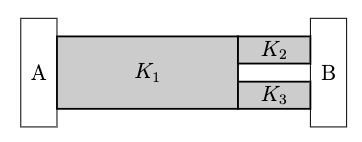
\includegraphics{picture_1.png}
        \end{center}

        Calculate the rate of heat flow through each rod and the temperature in the middle where $K_1$ is connected to the parallel combination of $K_2$ and $K_3$.

        \subsection{Solution}
            The best move here would be to calculate the equivalent heat conductence of the entire system.
            \begin{align}
                K_{23}  &=  K_2 + K_3\\
                K_{\rm eq}  &=  \left( \frac{1}{K_1} + \frac{1}{K_2 + K_3} \right)^{-1}
            \end{align}

            This can be multiplied by the change in temperature to get the heat flow along the entire system.
            \begin{align}
                \Delta T    &=  40\unit{\kelvin}\\
                \dv{Q}{t}   &=  K \cdot \Delta T
                    =   \left( \frac{1}{K_1} + \frac{1}{K_2 + K_3} \right)^{-1} * \Delta T\\
                    &=  \left( \frac{1}{100} + \frac{1}{125 + 175} \right)^{-1} * (40)
                    =   3000\,\unit{\watt}
            \end{align}

            This would equivalently be the rate at which the heat would flow through rod $K_1$, as well as the combination of rods two and three.
            It can also be first used to find the temperature at where $K_1$ is connected.
            \begin{align}
                \Delta T    &=  \frac{dQ/dt}{K_1}
                    =   \frac{3000}{100}
                    =   30\,\unit{\kelvin}\\
                T_{\rm middle}  &=  40\unit{\celsius} - 30\,\unit{\kelvin}
                    =   10\,\unit{\celsius}
            \end{align}

            This equivalently makes $\Delta T$ between the middle and system B equal to $-10\,\unit{\kelvin}$. 
            This in turn can be used to find the rate of heat flow along both $K_2$ and $K_3$.
            \begin{align}
                \left( \dv{Q}{t} \right)_2  &=  K_2 * \Delta T
                    =   125 * (10)
                    =   1250\,\unit{\watt}\\
                \left( \dv{Q}{t} \right)_3  &=  K_3 * \Delta T
                    =   175 * (10)
                    =   1750\,\unit{\watt}
            \end{align}

    \pagebreak
    \section{Problem 2}
        (2 points) A particular system executes a cyclical process whose P-V graph is a clockwise-directed ellipse centered at ($V_0$, $P_0$) and radii $\delta V$ and $\delta P$, respectively. 
        Calculate the net work done and the net heat flow into/out of this system during one cycle.
        \begin{center}
            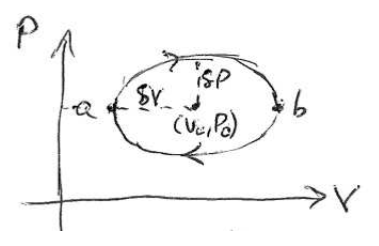
\includegraphics{picture_2.png}
        \end{center}

        \subsection{Solution}
            We know that the process is cyclical, so the net change in internal energy will be zero. 
            This, due to the first law of thermodynamics, means that the heat inserted is equal to the negative of the work done on the system, so we only have to calculate one of the two.
            To do this, we can set up an equation for the work done on the system.
            \begin{align}
                W   &=  -\int_{t_i}^{t_f} P(t)\,\dv{V(t)}{t}\,dt
            \end{align}

            From here, we could go about just brute-forcing an answer, but it would be easier just to calculate the area enclosed by the process.
            Said enclosure is an ellipse, which has radii $\delta V$ and $\delta P$. 
            \begin{align}
                A   &=  \pi ab
                    =   \pi * \delta V * \delta P
            \end{align}

            This can be inserted into our equation for $W$.
            \begin{align}
                W   &=  -A
                    =   -\pi * \delta V * \delta P
            \end{align}

            The work would be negative because it starts by going over then goes under, resulting in a net positive area from the integral and a net negative work.
            From this, we can use the net zero change in internal energy to get the energy gained as heat.
            \begin{gather}
                \Delta E_{\rm int} = 0 = Q_{\rm in} + W_{\rm in} \to Q_{\rm in} = -W_{\rm in}\\
                \boxed{Q_{\rm in} = \pi * \delta V * \delta P}\\
                \boxed{W_{\rm in} = -\pi * \delta V * \delta P}
            \end{gather}

            % There is an equation for the ellipse.
            % \begin{gather}
            %     \frac{\left( V(t) - V_0 \right)^2}{\delta V^2} + \frac{\left( P(t) - P_0 \right)^2}{\delta P^2} = 1
            % \end{gather}

            % We can solve this for $P(t)$ to get $P(V)$.
            % \begin{gather}
            %     \frac{\left( P(t) - P_0 \right)^2}{\delta P^2} = 1 - \frac{\left( V(t) - V_0 \right)^2}{\delta V^2}\\
            %     \frac{P(t) - P_0}{\delta P} = \pm \sqrt{ 1 - \frac{\left( V(t) - V_0 \right)^2}{\delta V^2} }\\
            %     P(t) - P_0 = \pm \delta P \sqrt{ 1 - \frac{\left( V(t) - V_0 \right)^2}{\delta V^2} }\\
            %     P(t) = P_0\,\pm\,\delta P \sqrt{ 1 - \frac{\left( V(t) - V_0 \right)^2}{\delta V^2} }\\
            %     P(V) = P_0\,\pm\,\delta P \sqrt{ 1 - \frac{\left( V - V_0 \right)^2}{\delta V^2} }
            % \end{gather}

            % This can be integrated.
            % Looking above at the equation for work, the left integral can be given the positive square root, while the right integral can be given the negative square root.
            % {\footnotesize
            % \begin{align}
            %     W   &=  -\int_{a}^{b} P(V)\,dV - \int_{b}^{a} P(V)\,dV\\
            %         &=  -\int_{a}^{b} P_0\,+\, \delta P \sqrt{ 1 - \frac{\left( V - V_0 \right)^2}{\delta V^2} }\,dV - \int_{b}^{a} P_0\,-\,\delta P \sqrt{ 1 - \frac{\left( V - V_0 \right)^2}{\delta V^2} }\,dV\\
            %         &=  \int_{b}^{a} P_0\,+\, \delta P \sqrt{ 1 - \frac{\left( V - V_0 \right)^2}{\delta V^2} }\,dV - \int_{b}^{a} P_0\,-\,\delta P \sqrt{ 1 - \frac{\left( V - V_0 \right)^2}{\delta V^2} }\,dV\\
            %         &=  \int_{b}^{a} P_0\,+\, \delta P \sqrt{ 1 - \frac{\left( V - V_0 \right)^2}{\delta V^2} } - P_0\,+\,\delta P \sqrt{ 1 - \frac{\left( V - V_0 \right)^2}{\delta V^2} }\,dV\\
            %         &=  \int_{b}^{a} \delta P \sqrt{ 1 - \frac{\left( V - V_0 \right)^2}{\delta V^2} }\,+\,\delta P \sqrt{ 1 - \frac{\left( V - V_0 \right)^2}{\delta V^2} }\,dV\\
            %         &=  \int_{b}^{a} 2 * \delta P \sqrt{ 1 - \frac{\left( V - V_0 \right)^2}{\delta V^2} }\,dV
            %         =   2 * \delta P \int_{b}^{a} \sqrt{ 1 - \frac{\left( V - V_0 \right)^2}{\delta V^2} }\,dV
            % \end{align}}

            % We can recall in this instance that $\dv{V} (V) = 1$, which we can insert into this.
            % \begin{align}
            %     W   &=   2 * \delta P \int_{b}^{a} \dv{V}{V} * \sqrt{ 1 - \frac{\left( V - V_0 \right)^2}{\delta V^2} }\,dV
            % \end{align}

            % Integration by parts is applicable here, with the following values in $u$ and $v$.
            % \begin{gather}
            %     \int u\dv{v}{x}\,dx = uv - \int v\dv{u}{x}\,dx\\
            %     \begin{align}
            %         &u  =   \sqrt{ 1 - \frac{ \left( V - V_0 \right)^2 }{ \delta V^2 } }
            %             &du =   \frac{\sqrt{2 (V - V_0) }}{2*\delta V \sqrt{1 - \frac{ \left( V - V_0 \right)^2}{\delta V^2} }}\\
            %         &v  =   V   
            %             &dv = 1
            %     \end{align}\\
            %     \begin{align}
            %         W   &=  2 * \delta P \int_{b}^{a} \sqrt{ 1 - \frac{\left( V - V_0 \right)^2}{\delta V^2} }\,dV\\
            %             &=  2\,\delta P \left( V \sqrt{ 1 - \frac{ \left( V - V_0 \right)^2 }{ \delta V^2 } } - \int_{b}^{a} V \frac{\sqrt{2 (V - V_0) }}{2*\delta V \sqrt{1 - \frac{ \left( V - V_0 \right)^2}{\delta V^2} }}\,dV \right)
            %     \end{align}
            % \end{gather}

            % We can focus on the integral in this equation.
            % \begin{gather}
            %     \int_{b}^{a} V \frac{\sqrt{2 (V - V_0) }}{2*\delta V \sqrt{1 - \frac{ \left( V - V_0 \right)^2}{\delta V^2} }}\,dV\\
            %     \frac{\sqrt{2}}{2 * \delta V} * \int_{b}^{a} V \frac{\sqrt{ V - V_0 }}{\sqrt{1 - \frac{ \left( V - V_0 \right)^2}{\delta V^2} }}\,dV\\
            %     % \frac{\sqrt{2}}{2 * \delta V} * \int_{(b - V_0)^2}^{(a - V_0)^2} \frac{1}{2} \frac{\sqrt{ u }}{\sqrt{1 - \frac{ u }{\delta V^2} }}\,dV\\
            %     % \frac{\sqrt{2}}{2 * \delta V} * \int_{(b - V_0)^2}^{(a - V_0)^2} \frac{\delta V}{2} \frac{\sqrt{ u }}{\sqrt{\delta V^2 - u }}\,dV\\
            %     % \frac{\sqrt{2}}{4} * \int_{(b - V_0)^2}^{(a - V_0)^2} \frac{\sqrt{ u }}{\sqrt{\delta V^2 - u }}\,dV\\
            % \end{gather}

            % We can use ths to solve for $V(t)$.
            % \begin{gather}
            %     \frac{\left( V(t) - V_0 \right)^2}{\delta V^2} + \frac{\left( P(t) - P_0 \right)^2}{\delta P^2} = 1\\
            %     \frac{\left( V(t) - V_0 \right)^2}{\delta V^2} = 1 - \frac{\left( P(t) - P_0 \right)^2}{\delta P^2}\\
            %     \left( V(t) - V_0 \right)^2 = \delta V^2 \left( 1 - \frac{\left( P(t) - P_0 \right)^2}{\delta P^2} \right)\\
            %     V(t) - V_0  =   \delta V \sqrt{ 1 - \frac{\left( P(t) - P_0 \right)^2}{\delta P^2} }\\
            %     V(t)    =   V_0 + \delta V \sqrt{ 1 - \frac{\left( P(t) - P_0 \right)^2}{\delta P^2} }\\
            %     \dv{V(t)}{t}    =   \dv{t} \left( V_0 + \delta V \sqrt{ 1 - \frac{\left( P(t) - P_0 \right)^2}{\delta P^2} } \right)\\
            %     \dv{V(t)}{t}    =   \delta V \dv{t} \left( \sqrt{ 1 - \frac{\left( P(t) - P_0 \right)^2}{\delta P^2} } \right)\\
            %     \dv{V(t)}{t}    =   \frac{\delta V \sqrt{ \dv{t} \left( - \frac{\left( P(t) - P_0 \right)^2}{\delta P^2} \right) } }{2 \left( \sqrt{ 1 - \frac{\left( P(t) - P_0 \right)^2}{\delta P^2} } \right)}\\
            %     \dv{V(t)}{t}    =   \frac{\frac{\delta V}{\delta P} \sqrt{ 2 \left( P(t) - P_0 \right) } }{2 \left( \sqrt{ 1 - \frac{\left( P(t) - P_0 \right)^2}{\delta P^2} } \right)} 
            % \end{gather}
    
    \pagebreak
    \section{Problem 3}
        (10 points) The left face of a rod at x = 0 (shown below) is fixed at a temperature of T(0) and the right face at x = L is fixed at a temperature of T (L). 
        The radius varies from a to b uniformly as x varies from 0 to L. The material has a thermal conductivity k which is the same throughout the entire volume.
        \begin{center}
            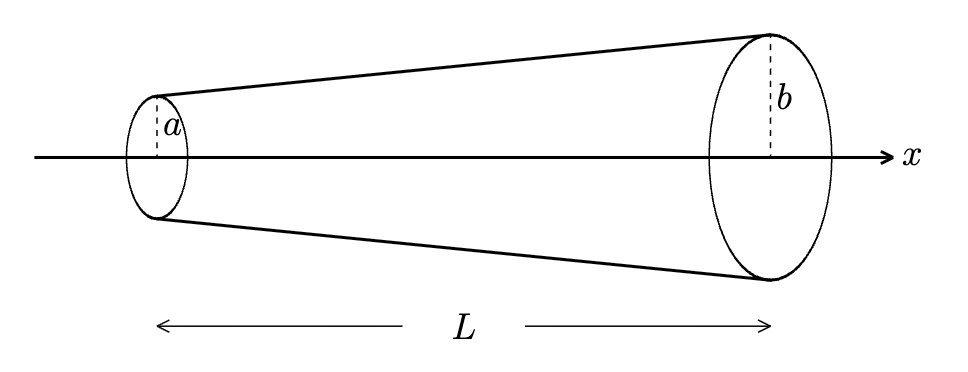
\includegraphics[width=\textwidth]{picture_3.png}
        \end{center}

        a. (4 points) Show that the temperature profile is given by
        \begin{equation*}
            T (x) - T (0) = - \frac{x}{k \pi ar}\dv{Q}{t}
        \end{equation*}
        where r is the radius at x. 
        Hint: Recall that $\dv{T}{x} = (-1/k \pi r^2)\dv{Q}{t}$. 
        This should be integrated over x, although the integral can be most easily done if you substitute $x \to r$.
        
        b. (2 points) Determine the thermal conductance of the entire rod.
        
        c. (4 points) If T(0) = 80\unit{\celsius}, T(L) = 20\unit{\celsius}, and $b = 2a$, calculate T(L/2).


        \subsection{Solution (a)}
            The first we can do is, as advised, use the differential equation. 
            \begin{gather}
                r   =   \frac{b - a}{L} x + a \to \frac{1}{r(x)} = \frac{L}{bx - ax + aL}\\
                r^2 =   \left( \frac{b - a}{L} x + a \right)^2
                    =   \left( \frac{bx - ax + aL}{L} \right)^2\\
                \dv{T}{x}   = -\frac{1}{k \pi r^2}\,\dv{Q}{t}
                    =   -\frac{1}{k \pi}\,\dv{Q}{t} * \frac{1}{r^2}
            \end{gather}

            We can find an equation for $\frac{1}{r^2}$.
            We can then take the derivative of our equation for $r$ with respect to $x$ to get a new differential equation.
            \begin{gather}
                \frac{1}{r^2}   =   \frac{L^2}{\left( bx - ax + aL \right)^2}\\
                \dv{r}{x}   =   \dv{x}\left( \frac{b - a}{L} x + a \right)
                    =   \frac{b - a}{L}\\
                dr  =   \frac{b - a}{L}\,dx\\
                dx  =   \frac{L}{b - a}\,dr
            \end{gather}

            This can be used in our equation for $\dv{T}{x}$, which can in turn be solved for $dT$.
            \begin{align}
                \dv{T}{x}   &=  -\frac{1}{k \pi}\,\dv{Q}{t} * \frac{1}{r^2}\\
                dT  &=  -\frac{1}{k \pi}\,\dv{Q}{t} * \frac{1}{r^2}\,dx\\
                    &=  -\frac{1}{k \pi}\,\dv{Q}{t} * \frac{1}{r^2} * \frac{L}{b - a}\,dr
            \end{align}

            This can in turn be integrated from r(0) to r($x$) and from T(0) to T($x$).
            \begin{gather}
                \int_{T(0)}^{T(x)}\,dT  =   T(x) - T(0)\\
                \begin{align}
                    T   &=  \int_{r(0)}^{r(x)} -\frac{1}{k \pi}\,\dv{Q}{t} * \frac{1}{r^2} * \frac{L}{b - a}\,dr
                        =   -\frac{1}{k \pi}\,\dv{Q}{t} * \frac{L}{b - a} * \int_{r(0)}^{r(x)} \frac{1}{r^2}\,dr\\
                        &=  -\frac{1}{k \pi}\,\dv{Q}{t} * \frac{L}{b - a} * \left[ -\frac{1}{r} \right]_{r(0)}^{r(x)}
                        =   \frac{1}{k \pi}\,\dv{Q}{t} * \frac{L}{b - a} * \left( \frac{1}{r(x)} - \frac{1}{r(0)} \right)\\
                        &=  \frac{1}{k \pi}\,\dv{Q}{t} * \frac{L}{b - a} * \left( \frac{L}{bx - ax + aL} - \frac{1}{a} \right)\\
                        &=  \frac{1}{k \pi}\,\dv{Q}{t} * \frac{L}{b - a} * \left( \frac{aL - bx + ax - aL}{a(bx - ax + aL)} \right)\\
                        &=  \frac{1}{k \pi}\,\dv{Q}{t} * \frac{L}{b - a} * \left( \frac{-bx + ax}{a(bx - ax + aL)} \right)\\
                        &=  -\frac{1}{k \pi}\,\dv{Q}{t} * \frac{Lx}{a(bx - ax + aL)}
                \end{align}
            \end{gather}

            From the latter, we can now substitute for extrapolated locations of $r$ given the values we found above. 
            \begin{align}
                T   &=  -\frac{1}{k \pi}\,\dv{Q}{t} * \frac{Lx}{a\left( \left( \frac{b - a}{L}x \right)L + aL \right)}
                    =   -\frac{1}{k \pi}\,\dv{Q}{t} * \frac{\cancel{L}x}{a\cancel{L}\left( \frac{b - a}{L}x + a \right)}\\
                    &=  -\frac{1}{k \pi}\,\dv{Q}{t} * \frac{x}{ar}
                    =   -\frac{x}{k \pi ar}\,\dv{Q}{t}
            \end{align}

            Put the two integrals together to get the equation by transistive property.
            \begin{equation}
                \boxed{T(x) - T(0)  =   -\frac{x}{k \pi ar}\,\dv{Q}{t}}
            \end{equation}

        \subsection{Solution (b)}
            The thermal conductance $K$ is describable from an equation.
            \begin{gather}
                \dv{Q}{t}   =   K\,\Delta T
            \end{gather}

            We can see a similarity with our equation for the temperature profile and use algebra to make it look like the equation involving thermal conductance.
            For one thing, $T(x) - T(0)$ can be turned into $\Delta T$, especially because we will be setting $x = L$ since we are considering the entire rod.
            On that note, the value of $r$ will be determinable by our prior equation $\frac{b - a}{L}x + a$. 
            \begin{gather}
                r(L)    =   \frac{b - a}{L} * L + a
                    =   b - a + a
                    =   b\\
                T(L) - T(0) =   \Delta T
                    =   -\frac{x}{k \pi ar}\,\dv{Q}{t}
                    =   -\frac{L}{k \pi ab}\,\dv{Q}{t}\\
                -\frac{k \pi ab}{L}\Delta T =   \dv{Q}{t}
            \end{gather}

            Given the position and the prior necessary value of $K$, our conductance would be $-\frac{k \pi ab}{L}$.
            Since thermal conductance is always positive, we would take the absolute value for our final answer.
            \begin{equation}
                \boxed{K = \frac{k \pi ab}{L}}
            \end{equation}
        
        \subsection{Solution (c)}
            For starters, calculate $r(x)$ given that $b = 2a$.
            \begin{align}
                r(x)    &=  \frac{b - a}{L}x + a
                    =   \frac{2a - a}{L}x + a
                    =   \frac{a}{L}x + a
            \end{align}

            We can from here create two separate equations, one where $x = L$ and the other where $x = \frac{L}{2}$.
            \begin{gather}
                T(L) - T(0) =   -\frac{x}{k \pi ar(L)}\,\dv{Q}{t}\\
                T(L/2) - T(0)   =   -\frac{x}{k \pi ar(L/2)}\,\dv{Q}{t}
            \end{gather}

            We can separate the identicals and the non-identicals into something we can use transistivity on.
            Start with where $x = L$.
            \begin{gather}
                T(L) - T(0) =   -\frac{L}{k \pi ar(L)}\,\dv{Q}{t}\\
                (T(L) - T(0)) * \frac{r(L)}{L} =   -\frac{1}{k \pi a}\,\dv{Q}{t}
            \end{gather}

            Then where $x = L/2$.
            \begin{gather}
                T(L/2) - T(0) =   -\frac{x}{k \pi ar(L/2)}\,\dv{Q}{t}\\
                (T(L/2) - T(0)) * \frac{r(L/2)}{L/2} =   -\frac{1}{k \pi a}\,\dv{Q}{t}
            \end{gather}

            This is the point we can use transistivity on.
            We can also sub in the equation for $r(x)$ at some point.
            {   \small
            \begin{gather}
                (T(L) - T(0)) * \frac{r(L)}{L} = (T(L/2) - T(0)) * \frac{r(L/2)}{L/2}\\
                (T(L) - T(0)) * \frac{1}{L} * \left( \frac{a}{L} * L + a \right) = (T(L/2) - T(0)) * \frac{2}{L} * \left( \frac{a}{L} * \frac{L}{2} + a \right)\\
                (T(L) - T(0)) * \left( a + a \right) = (T(L/2) - T(0)) * 2 * \left( \frac{a}{2} + a \right)\\
                (T(L) - T(0)) * 2 = (T(L/2) - T(0)) * 2 * \frac{3}{2} = (T(L/2) - T(0)) * 3\\
                (T(L) - T(0)) * \frac{2}{3} = T(L/2) - T(0)\\
                T(L/2)  =   (T(L) - T(0)) * \frac{2}{3} + T(0)
            \end{gather}    }

            This gives us a final equation we can sub in for to get our final answer.
            \begin{align}
                T(L/2)  &=  (T(L) - T(0)) * \frac{2}{3} + T(0)
                    =   (20\unit{\celsius} - 80\unit{\celsius}) * \frac{2}{3} + 80\unit{\celsius}\\
                    &=  -60\,\unit{\celsiusdegree} * \frac{2}{3} + 80\unit{\celsius}
                    =   -40\,\unit{\celsiusdegree} + 80\unit{\celsius}
                    =   \boxed{40\unit{\celsius}}
            \end{align}
\end{document}